\section{{\xstate}: Try-Catch Statement Detector}
\label{interpretation:sec}

{\xstate} also uses CodeBERT, the same one as in {\xblock}. However, we create a separate figure for each module so that it is easier to follow. 

Each \texttt{[SEP]} token represents the line of code preceding it (Note that semicolon would not be as consistent a line separator as the \texttt{[SEP]} token, since a line of code may not end with a semicolon. And a semicolon often appears inside string literals and inside for-loop conditions. ). We expect that the relationship between lines of code can be learnt through these \texttt{[SEP]} tokens during training, so that at prediction time, the model can determine for each line as to whether it is inside or outside a try-catch block. We devise three tags in the IOB2 format to accomplish this task: \texttt{O} tag means that the statement is outside any try-blocks; \texttt{B-Try} tag means the statement begins a try-block; and \texttt{I-Try} tag means the statement is inside a try-block and is not the first line in that try-block. 

During training, tags of all the lines are known from the code. During prediction, the model will be able to assign tags to all the lines in the code snippet. From these tags, we get to know how many try-blocks should be added, and which lines of code belong to which try-block.



% This section presents {\xstate} and how we leverage an Explainable AI
% model, GNNExplainer~\cite{GNNExplainer}, to detect what statements in
% the given code snippet $C$ need to be placed in a \code{try-catch} block
% provided that {\xblock} had decided the necessity of such a block.

% %Tien
% {\xstate} takes the following as inputs: 1) the PDG ($G_C$) of the
% given code $C$, 2) the trained R-GCN model for {\xblock}, along with
% the positive detection result $\mathcal{V_C}$ and the prediction score.
% Figure~\ref{fig:GNNEX} displays an illustration of the process in
% {\xstate}.

% % Let us explain how we use GNNExplainer~\cite{GNNExplainer} to build
% %our graph-based interpretation. The input includes the trained FA-GCN
% %model, the PDG ($G_M$) of the method $M$, and the detection result
% %$\mathcal{V}$ or $\mathcal{NV}$, and prediction score.

% %Figure~\ref{fig:GNNEX} illustrates our process for the case of
% %$\mathcal{V}$ (Vulnerable) (the case of $\mathcal{NV}$ is done
% %similarly).



% %The interpretations include 1) a crucial sub-graph $\mathcal{G}_M$,
% %corresponding to the PDG sub-graph consisting of statements relevant
% %to the vulnerability, and 2) a subset of crucial features
% %$\mathcal{X}_M$, corresponding to the set of variables involving to
% %the vulnerability.

% To decide the statements in the given code to be placed in a
% \code{try-catch} block, we aim to determine the statements that are
% most decisive and crucial for the {\xblock} model in deciding its
% outcome of ``Yes'' (i.e, {\xblock} decides that the snippet must be
% placed in a \code{try-catch} block). Therefore, we formulate that as
% the following problem: finding a sub-graph $\mathcal{G}_C$ in the PDG
% $G_C$ for $C$ that minimizes the difference in the prediction scores
% between using the entire graph $G_C$ and using the minimal graph
% $\mathcal{G}_C$. To do so, we leverage the Explainable AI model,
% GNNExplainer~\cite{GNNExplainer}. It uses a masking technique in which
% instead of searching for that minimal subgraph, it learns the {\em
%   edge-mask} set $EM$ of the edges and the {\em feature-mask} set $FM$
% of the features. Learning those two sets $EM$ and $FM$ helps derive
% the explanation sub-graph $\mathcal{G}_C$ and the set of crucial
% feature $\mathcal{X}_C$ by masking-out the edges in $EM$ from $G_C$,
% and the feature in $FM$ from $X_C$:
% \begin{equation}\label{eq:11}
% \mathcal{G}_C = G_C \bigodot EM
% \end{equation}
% \begin{equation}\label{eq:12}
% \mathcal{X}_M = X_M \bigodot FM
% \end{equation}
% $\bigodot$ is used to denote the ``masking-out'' operation.

% %To derive the interpretations, the key goal is to find a sub-graph
% %$\mathcal{G}_M$ in the PDG $G_M$ of the method $M$ that minimizes the
% %difference in the prediction scores between using the entire graph
% %$G_M$ and using the minimal graph $\mathcal{G}_M$. To do so, we use
% %GNNExplainer with the {\em masking technique}~\cite{GNNExplainer},
% %which treats the searching for the minimal graph $\mathcal{G}_M$ as a
% %learning problem of the {\em edge-mask} set $EM$ of the edges.  The
% %idea is that learning $EM$ helps {\tool} derive the interpretation
% %sub-graph $\mathcal{G}_M$ by masking-out the edges in $EM$ from $G_M$
% %(``masked-out'' is denoted by
% %$\bigodot$): \begin{equation}\label{eq:11} \mathcal{G}_M = G_M
% %\bigodot EM \end{equation}

% Figure~\ref{fig:GNNEX} illustrates the principle. Note that the
% trained R-GCN model in {\xblock} had decided that a \code{try-catch}
% block is needed for the given code (in which the entire original PDG
% was used as input). When an edge-mask set is applied, some of the
% edges (and the inducing nodes) are masked. With the new graph being
% used as~the new input, if the trained R-GCN model in {\xblock}
% produces ``Yes'' as the result, i.e., {\em the classification does not
% change, then the edges in the edge-mask set are not important}. Thus,
% they will not be included in the explanation graph $\mathcal{G}_C$. If
% the trained R-GCN model in {\xblock} with the new input graph produces
% ``No'' as the result, i.e., {\em the classification does change from
% ``Yes'' to ``No'', then those edges in the edge-mask set are important
% to the model, thus, being included in the explanation graph
% $\mathcal{G}_C$}. Similar logic is applied to include or exclude the
% features in the {\em feature-mask} $FM$.



% %Tien Figure~\ref{fig:GNNEX} illustrates GNNExplainer's principle. As
% %an edge-mask set is applied, GNNEXplainer checks if the FA-GCN model
% %produces the same result~(in this case the result is
% %$\mathcal{V}$). If yes, the edge in the edge-mask is not important
% %and is not included in $\mathcal{G}_M$. Otherwise, the edge is
% %important and included in $\mathcal{G}_M$.  Because the numbers of
% %possible sub-graphs and the edge-mask sets are untractable,
% %GNNExplainer uses a learning approach for the edge-mask $EM$.

% %\begin{equation}\label{eq:12}
% %\mathcal{X}_M = X_M \bigodot FM
% %\end{equation}

% %For example, as you can see in figure \ref{fig:GNNEX}, when the
% %GNNExplainer get the whole PGD $G_m$, it starts to use the
% %\textit{edge-mask} $EM$ and \textit{feature-mask} $FM$ to mask some
% %edges and features.  As you can see in the second row of the figure,
% %after masked some edges from $G_m$ to generate a graph $G'_m$,
% %GNNExplainer use the detection model to check the new graph to see
% %how the detection result changes. If the result has been influenced a
% %lot, it means that the masked edges are important for the detection
% %result. If not, it means that the masked edges are not important for
% %the detection result. It is similar for the \textit{feature-mask}
% %$FM$.  Because in the last step, we could get $F_{v}$ for each
% %statement $v$ and $F_{v}$ have the same dimension, $FM$ masks the
% %features in the same position in $F_{v}$ for each statement $v$ and
% %then use detection model to evaluate the importance of the masked
% %features just as the edges. As you can see in figure \ref{fig:GNNEX},
% %$FM$ masked the second and the 4th feature for each statement in this
% %example.

% \begin{figure}[t]
% 	\centering
% 	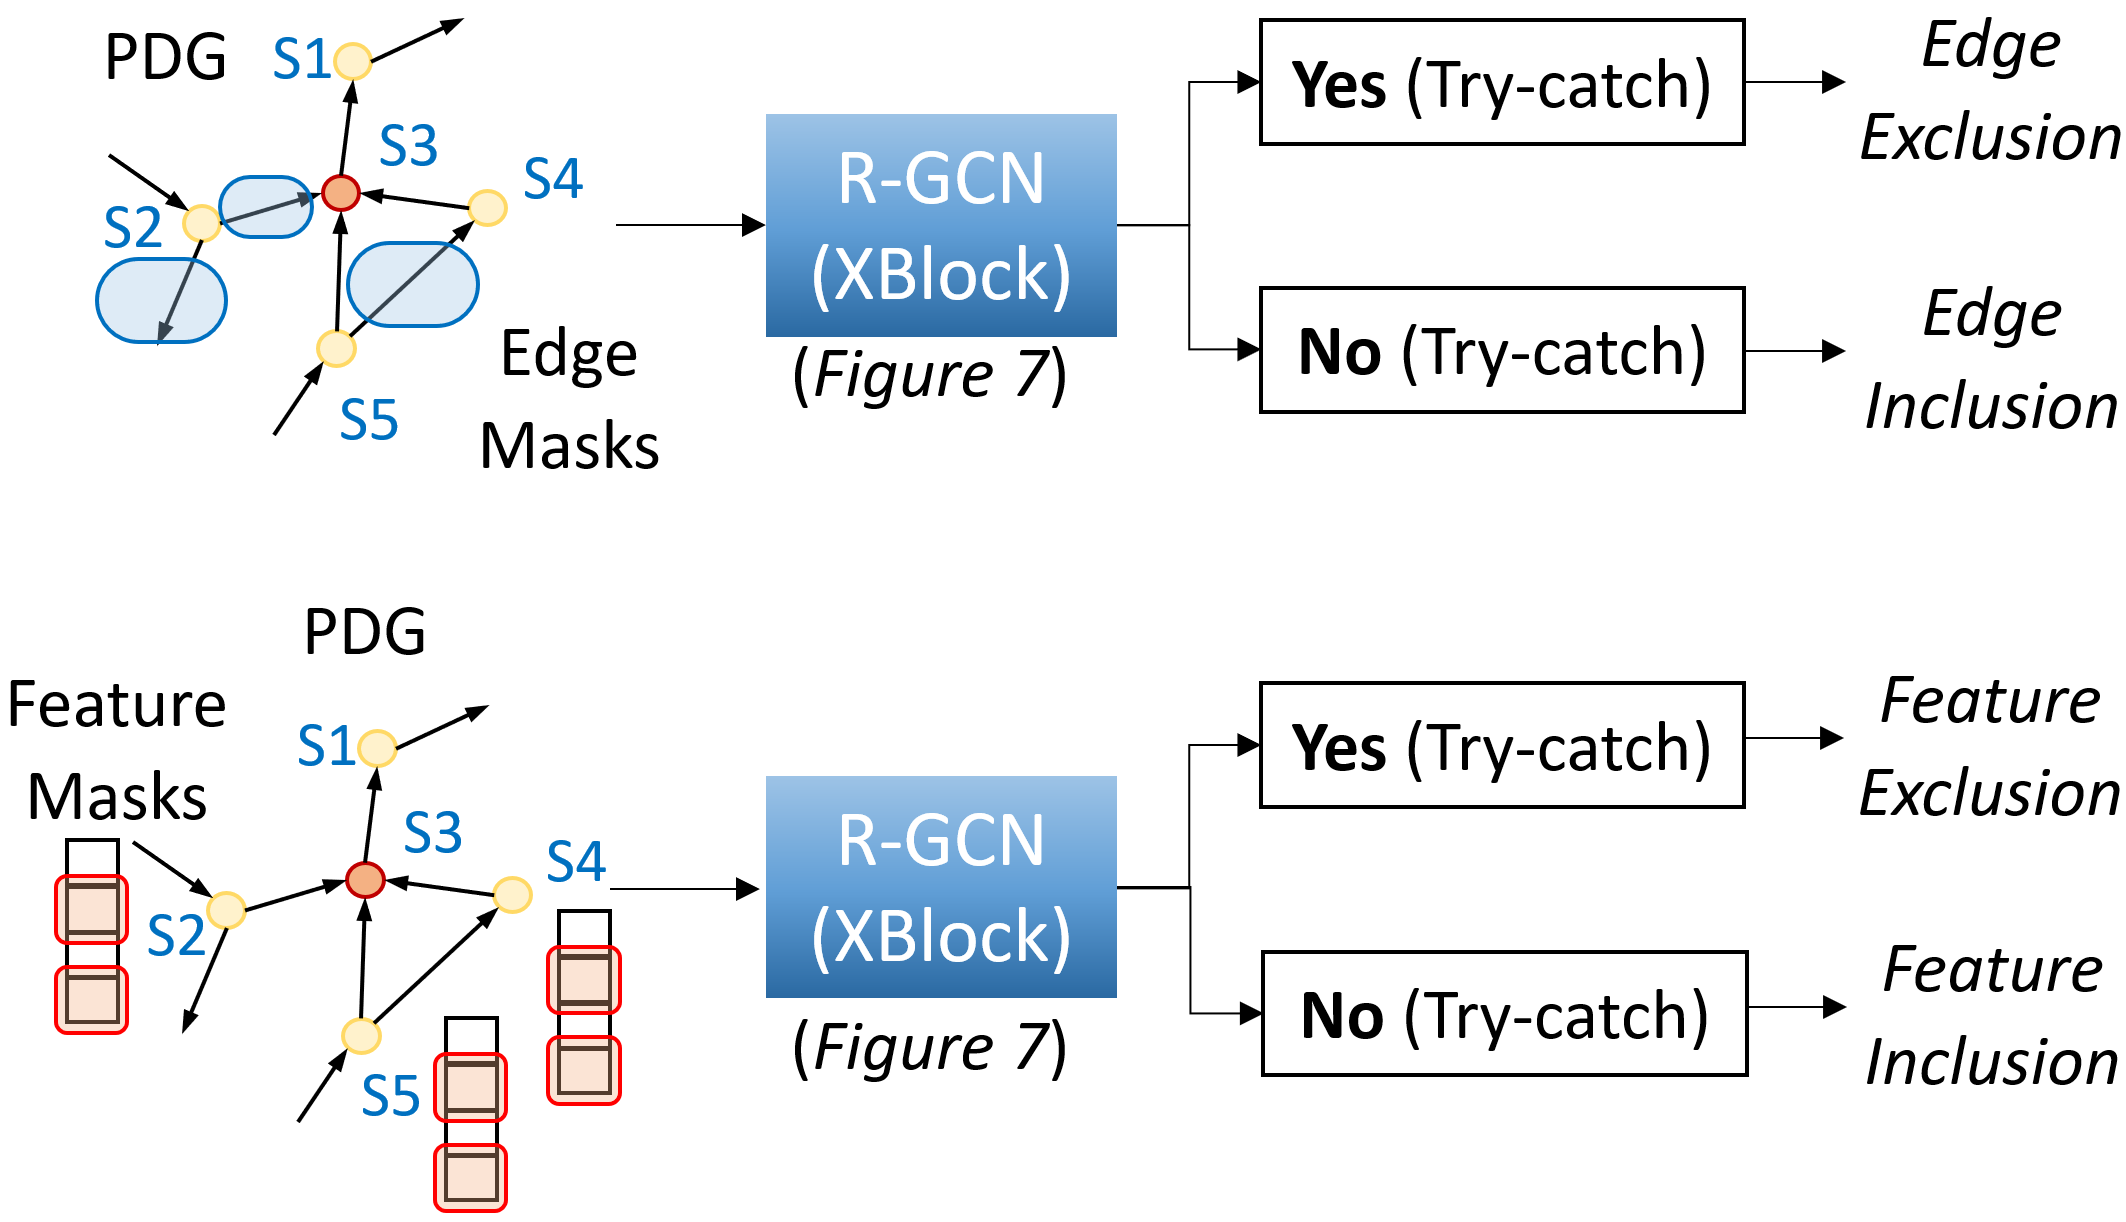
\includegraphics[width=3in]{XAI.png}
%         \vspace{-0.06in}
% 	\caption{Masking to derive the explanation sub-graph containing statements in a \code{Try-Catch} block ({\xstate})}
%         \vspace{-0.06in}
% 	\label{fig:GNNEX}	
% \end{figure}

% %\begin{align}\label{maineq}
% %\nonumber
% %\max_{\mathcal{G}_M} MI(Y,(\mathcal{G}_M,\mathcal{X}_M)) = H(Y) - H(Y|G=\mathcal{G}_M,X=\mathcal{X}_M)
% %\end{align}

% %to minimizing conditional entropy
% %$H(Y|G=\mathcal{G}_M,X=\mathcal{X}_M)$

% %\begin{equation}
% %  \label{eq2}
% %-\EX_{Y|\mathcal{G}_M,
% %  \mathcal{X}_M} [log P_{FA-GCN} (Y|G=\mathcal{G}_M,X=\mathcal{X}_M)]
% %  \end{equation}

% %\begin{equation}
% %  \label{eq3}
% %  \min_{\mathcal{G}} \EX_{\mathcal{G}_M \sim \mathcal{G}} H(Y|G=\mathcal{G}_M,X=\mathcal{X}_M)
% %\end{equation}
% %\begin{equation}
% %  \label{eq4}
% %  \min_{\mathcal{G}} H(Y| G=\EX_{\mathcal{G}}[\mathcal{G}_M], X=\mathcal{X}_M)
% %\end{equation}
% %\nonumber

% Because the numbers of possible sub-graphs, edge-mask sets, and
% feature-mask sets are untractable, GNNExplainer uses a learning
% approach for $EM$ and $FM$. It aims to maximize the mutual information
% (MI) between the minimal graph $\mathcal{G}_C$ and the input
% PDG~$G_C$~\cite{GNNExplainer}:
% \begin{equation}\label{maineq}
% \max_{\mathcal{G}_C} MI(Y,\mathcal{G}_C) = H(Y) - H(Y|G=\mathcal{G}_C)
% \end{equation}
% $Y$ is the outcome decision by the trained R-GCN model. Thus, the
% entropy term $H(Y)$ is constant for the trained R-GCN
% model.

% Maximizing the $MI$ value for all $\mathcal{G}_C$s is equivalent
% to minimizing conditional entropy $H(Y|G=\mathcal{G}_C)$, which by
% definition of conditional entropy can be expressed~as
% \begin{equation}
%   \label{eq2}
% -\EX_{Y|\mathcal{G}_C}
%   [log P_{R-GCN} (Y|G=\mathcal{G}_C)]
% \end{equation}
% This conditional entropy is a measure of how
% much uncertainty remains about the outcome $Y$ when we know
% $G=\mathcal{G}_C$.
% %
% %GNNEXplainer also limits the size of $\mathcal{G}_C$ by $K_C$, {\em
% %  i.e.}, taking $K_C$ edges that give the highest mutual information
% %with the prediction outcome $Y$.
% %
% %Direct optimization of the formula(~\ref{eq2}) is not tractable, thus,
% %GNNExplainer treats $\mathcal{G}_C$ as a random graph variable
% %$\mathcal{G}$. The objective in Equation(~\ref{eq2}) becomes:
% %\begin{equation}
% %  \label{eq3}
% %  \min_{\mathcal{G}} \EX_{\mathcal{G}_C \sim \mathcal{G}} H(Y|G=\mathcal{G}_C)
% %\end{equation}
% %\begin{equation}
% %  \label{eq4}
% %  \min_{\mathcal{G}} H(Y| G=\EX_{\mathcal{G}}[\mathcal{G}_C])
% %\end{equation}
% %From Equation~\ref{eq3}, we obtain Equation~\ref{eq4} with Jensen's
% %inequality.  The conditional entropy in Equation~\ref{eq4} can be
% %optimized by replacing $\EX_{\mathcal{G}}[\mathcal{G}_C]$ to be
% %optimized by masking with $EM$ on the input graph $G_C$.  Now, we can
% %reduce the problem to learning the mask $EM$.  Similar logic is
% %applied to $FM$.

% More details can be found in~\cite{GNNExplainer}. The resulting
% sub-graph $\mathcal{G}_C$ is used to derive the statements to be
% placed in a \code{try-catch} block. Note that, we can set the
% statements to be consecutive.
